\let\negmedspace\undefined
\let\negthickspace\undefined
\documentclass[journal]{IEEEtran}
\usepackage[a5paper, margin=10mm, onecolumn]{geometry}
%\usepackage{lmodern} % Ensure lmodern is loaded for pdflatex
\usepackage{tfrupee} % Include tfrupee package

\setlength{\headheight}{1cm} % Set the height of the header box
\setlength{\headsep}{0mm}     % Set the distance between the header box and the top of the text

\usepackage{gvv-book}
\usepackage{gvv}
\usepackage{cite}
\usepackage{amsmath,amssymb,amsfonts,amsthm}
\usepackage{algorithmic}
\usepackage{graphicx}
\usepackage{textcomp}
\usepackage{xcolor}
\usepackage{txfonts}
\usepackage{listings}
\usepackage{enumitem}
\usepackage{mathtools}
\usepackage{gensymb}
\usepackage{comment}
\usepackage[breaklinks=true]{hyperref}
\usepackage{tkz-euclide} 
\usepackage{listings}
\usepackage{gvv}                                        
\def\inputGnumericTable{}                                 
\usepackage[latin1]{inputenc}                                
\usepackage{color}                                            
\usepackage{array}                                            
\usepackage{longtable}                                       
\usepackage{calc}                                             
\usepackage{multirow}                                         
\usepackage{hhline}                                           
\usepackage{ifthen}                                           
\usepackage{lscape}
\usepackage{circuitikz}
\tikzstyle{block} = [rectangle, draw, fill=blue!20, 
    text width=4em, text centered, rounded corners, minimum height=3em]
\tikzstyle{sum} = [draw, fill=blue!10, circle, minimum size=1cm, node distance=1.5cm]
\tikzstyle{input} = [coordinate]
\tikzstyle{output} = [coordinate]


\begin{document}

\bibliographystyle{IEEEtran}
\vspace{3cm}

\title{10.6.4}
\author{EE25BTECH11049 - Sai Krishna Bakki}
\maketitle
\vspace{-3em}
% \newpage
% \bigskip
{\let\newpage\relax\maketitle}

\renewcommand{\thefigure}{\theenumi}
\renewcommand{\thetable}{\theenumi}
\setlength{\intextsep}{10pt} % Space between text and floats


\numberwithin{equation}{enumi}
\numberwithin{figure}{enumi}
\renewcommand{\thetable}{\theenumi}

\textbf{Question:}\\
Draw a circle of radius 5cm. From a point 8cm away from its centre, construct a pair of tangents to the circle.\\
\solution\\
Let's take center as origin $\vec{O}$ and a point 8cm aways from its center as $\vec{h}=\myvec{8\\0}$.\\
The equation of a circle is given by 
\begin{align}
    g\brak{\vec{x}}=\norm{\vec{x}}^2+2\vec{u}^T\vec{x}+f=0
\end{align}
for
\begin{align}
\textbf{center}=\myvec{0\\0}, \text{since } \vec{c}=\vec{-u} 
\end{align}
we get
\begin{align}
\vec{u}=\myvec{0\\0}
\end{align}
we also know for any circle
\begin{align}
    \vec{V}=\myvec{1&0\\0&1}
\end{align}
radius(r) = 5cm, we know that  $r^2=\norm{u}^2-f$ which gives us 
\begin{align}
    f=-25
\end{align}
By using below equation, we can determine the direction vectors of the tangent lines from an external point
\begin{align} \vec{m}^T\sbrak{\brak{\vec{V}\vec{h}+\vec{u}}\brak{\vec{V}\vec{h}+\vec{u}}^T-\vec{V}g\brak{\vec{h}}}\vec{m}=0\\
g\brak{h}=39
\label{eq:tangent}
\end{align}
where $\vec{m}=\myvec{m_x\\m_y}$ is the direction vectors of a tangent line.\\
Substituting values in $\eqref{eq:tangent}$, we get
\begin{align}
\myvec{m_x&m_y}\myvec{25&0\\0&-39}\myvec{m_x\\m_y}=0\\
25m_x^2-39m_y^2=0\\
\end{align}
The slopes of the tangent line is given by $k=\frac{d_x}{d_x}$. we solve for the slopes:
\begin{align}
    k^2=\frac{25}{39}\implies k=\pm\frac{5}{\sqrt{39}}
\end{align}
Now, normal vectors of tangent lines are
\begin{align}
    \vec{n_1}=\myvec{5\\ \sqrt{39}},\vec{n_2}=\myvec{5\\ -\sqrt{39}}
\end{align}
Equations of tangent lines which passes through a point 8cm away from the center are
\begin{align}
    \vec{n_1^T}\vec{x}=c,\vec{n_2^T}\vec{x}=c
\end{align}
substituting $\vec{h}$ in line equation to get c,we get
\begin{align}
    c=40\\
    \myvec{5&\sqrt{39}}\vec{x}=40\\
    \myvec{5&-\sqrt{39}}\vec{x}=40
\end{align}
Now, solve for points of contact, for that we use the following formulae
\begin{align}
    \vec{q_i}=\brak{\pm r\brak{\frac{\vec{n_i}}{\norm{\vec{n_i}}}}-\vec{u}}
\end{align}
we get
\begin{align}
    \vec{q_1}=\myvec{\frac{25}{8}\\\frac{5\sqrt{39}}{8}},
    \vec{q_2}=\myvec{\frac{25}{8}\\-\frac{5\sqrt{39}}{8}}
\end{align}
\newpage
    \begin{figure}
    \centering
    \caption{}
    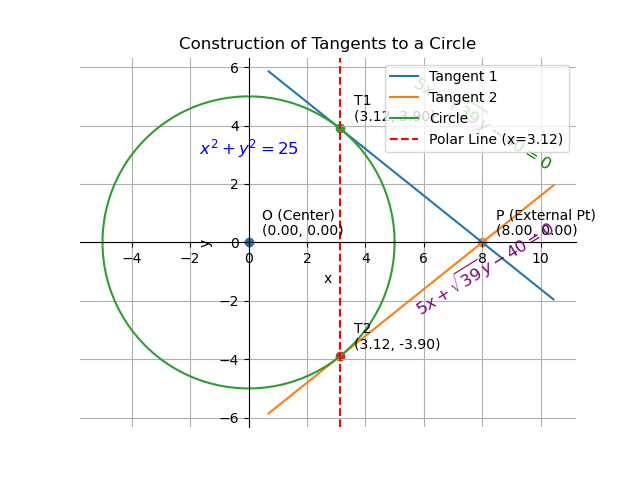
\includegraphics[width=0.9\columnwidth]{figs/Figure_1.png}
    \label{fig:placeholder}
\end{figure}
\end{document}